% !Mode:: "Tex:UTF-8"
\chapter{绪论}
\label{chap:1}

通讯和多媒体应用是半导体工业的主要推动力。
这两个领域日新月异的发展,
带来了对传输带宽永无止境的追求。
常见的高性能传输协议,
如以太网\upcite{IEEE8023_S4}、InfiniBand\upcite{InfiniBand}和PCI Express\upcite{pcie21}等,
其单通道带宽从本世纪初的3.125Gbps增长到目前的25Gbps。

为了克服在高频信号衰减方面的挑战,
每一代新的传输标准都会采用全新的编码方案。
因此,在通讯和多媒体芯片设计项目中,
最为关键且困难的工作之一是设计和验证特定的物理层编码器和解码器。
针对这一关键而困难的工作,
工业界常见的设计方法仍然停留在简单地手工编写代码,
并使用动态模拟器进行验证的阶段。

而随着传输带宽的进一步提升,
对于编码后信号01平衡和游程长度的统计特性要求也日益严格\upcite{encode6466}。
这就导致了在编码器中引进了更为复杂的,
包含大量异或操作的线性移位寄存器组,
如以太网标准clause 49的64/66加扰器\upcite{encode6466}和PCI Express标准的128/130编码器\upcite{pcie}。
大量的异或操作使得编码器的映射表非常不规则,
包含的corner case的数量随编码长度指数增长。
这就对传统的动态模拟验证方法的完备性提出了严峻挑战。

为此,
国防科技大学的Shen et al.\upcite{ShenICCAD09}于2009年首次提出了对偶综合的概念和基本的算法实现,
以从一个通讯协议的编码器源代码中,
自动产生其对应的解码器代码。
以此为起点,
集成电路设计自动化领域的研究者们在该领域取得了大量的研究成果\upcite{ShenICCAD09,ShenTCAD10,DBLP:conf/fmcad/ShenQZL10,ShenTCAD11,ShenICCAD11,ShenTCAD12,LiuICCAD11,LiuTCAD12,TuDAC13}。

在本章的剩余部分中,
我们将首先在小节\ref{sec_back}介绍相关的背景知识。
然后在小节\ref{sec_now}详细描述目前在该领域的研究成果。
然后在小节\ref{sec_whiteboxtodo}介绍基于白盒模型的对偶综合的研究意义和所面临的挑战。
最后在小节\ref{sec_contest_innov}介绍本文的研究内容和创新点。
\upcite{DBLP:conf/memocode/QinSJ14,DBLP:conf/apweb/QinSKD14}


\section{背景知识}\label{sec_back}
本节将给出相关的背景知识。

\subsection{基本记法}
布尔集合记为$B=\{0,1\}$。
多个变量组成的向量记为$\vec{v}=(v,\dots)$。
$\vec{v}$中的变量个数记为$|\vec{v}|$。
如果$v$是$\vec{v}$的成员,
则记为$v\in\vec{v}$;
否则$v\notin\vec{v}$。
对于变量$v$和向量$\vec{v}$,
如果$v\notin\vec{v}$,
则同时包含$v$和所有$\vec{v}$的成员的新向量记为$v\cup\vec{v}$。
如果$v\in \vec{v}$,
则包含所有$\vec{v}$的成员而不包含$v$的新向量记为$\vec{v}-v$。
对于两个向量$\vec{a}$和$\vec{b}$,
包含$\vec{a}$和$\vec{b}$的所有成员的新向量记为$\vec{a}\cup\vec{b}$。
向量$\vec{v}$的赋值集合记为$[\![\vec{v}]\!]$。
例如:
$[\![(v_1,v_2)]\!]=\{(0,0),(0,1),(1,0),(1,1)\}$。

在变量集合$V$上的布尔逻辑公式$F$是通过以下连接符连接$V$上的变量得到的:
包括$\neg$, $\wedge$,$\vee$和$\Rightarrow$,
他们分别代表着求反,与,或和蕴含操作。

\subsection{命题逻辑可满足性问题}

对在变量集合$V$上的布尔逻辑公式$F$,
命题逻辑可满足问题(缩写为SAT)
意味着寻找$V$的赋值函数$A:V\to B$,
使得$F$ 可以取值为$1$。
如果存在这样的赋值函数$A$,
则$F$ 是可满足的;
否则,
是不可满足的。

一个寻找上述赋值函数$A$的计算机程序称为SAT 求解器,
常见的SAT求解器包括Zchaff\upcite{CHAFF},
Grasp\upcite{grasp},
Berkmin\upcite{BERKMIN},
和MiniSat\upcite{EXTSAT}。


通常,
SAT 求解器要求有待求解的公式使用合取范式(CNF)表示,
其中一个公式是一个短句集合的合取,
一个短句是一个文字集合的析取,
一个文字是一个变量或者其反。
一个使用CNF 格式表示的公式通常也称为SAT 实例。


从文献\upcite{EFFSATUSMCCO}可知,
对于函数$f(v_1\dots v\dots v_n)$,
针对变量$v$的\textbf{正余因子}(cofactor)和\textbf{负余因子}分别是$f_{v\equiv 1}=f(v_1\dots 1\dots v_n)$ 和$f_{v\equiv 0}=f(v_1\dots 0\dots v_n)$。
而\textbf{余因子化}则代表着将1或者0赋予$v$以得到$f_{v\equiv 1}$ 和$f_{v\equiv 0}$。

给定两个布尔逻辑公式$\phi_A$ 和$\phi_B$,
若$\phi_A\wedge \phi_B$ 不可满足,
则存在仅使用了$\phi_A$ 和$\phi_B$共同变量的公式$\phi_I$ ,
 使得$\phi_A\Rightarrow \phi_I$且
$\phi_I\wedge \phi_B$不可满足。
$\phi_I$ 被称为$\phi_A$针对$\phi_B$的Craig插值\upcite{Craig}。
$\phi_I$可以使用McMillan算法\upcite{interp_McMillan}得到。
Craig插值通常被用于产生$\phi_A$的上估计。

\subsubsection{Tseitin编码}\label{subsubsec_tseitin}
在硬件验证过程中,
电路和属性通过Tseitin编码\upcite{Tseitin}转换为CNF公式,
而后交给SAT求解器求解。

任意电路均可以被表示为AND2门和INV 门的组合形式,
因此我们在这里仅给出AND2门和INV门的编码:
\begin{enumerate}
\item 对于非门INV $z=\neg x$,
由Tseitin编码产生的CNF公式为$(x\vee z)\wedge( \neg x\vee \neg z)$。
\item 对于二输入与门AND2 $z=x_1\wedge x_2$,
由Tseitin编码产生的CNF公式为$( \neg x_1\vee \neg x_2\vee z)\wedge(x_1\vee \neg z) \wedge(x_2\vee \neg z)$。
\item 对于一个表示为AND2门和INV门组合的复杂电路$C$,
由Tseitin编码产生的CNF公式$Tseitin(C)$ 是所有这些门的Tseitin编码的合取。
\end{enumerate}

包含一个INV门$d=\neg a$和一个AND2的$e=d\wedge c$的简单电路$C$,
他的Tseitin编码显示在公式(\ref{eqn_andinv})中。
\begin{multline}\label{eqn_andinv}
% \begin{equation}\label{eqn_andinv}
Tseitin(C)=
\left\{
\begin{array}{cc}
& (a\vee d) \\
\wedge & (\neg a\vee \neg d)
\end{array}
\right\}\wedge\left\{
\begin{array}{cc}
& (\neg e\vee c) \\
\wedge & (\neg e\vee d) \\
\wedge & (e\vee \neg c\vee\neg d)
\end{array}
\right\}
% \end{equation}
\end{multline}


%\subsection{SAT问题求解}
%确定SAT问题可满足赋值的计算,称为SAT求解。
%多数时候,可以使SAT问题可以满足的解并不是唯一的,求出所有可满足解被称为ALLSAT求解。

\subsubsection{SAT问题的简单解法}
为了方便对SAT求解过程的描述,
我们以图\ref{basic_circuit}中的电路为例子,
首先给出一个简单低效但是直观的求解方法。
并在下面逐步描述对该方法的改进措施,
从而最终描述清楚现代SAT求解器中常用的高效算法。

\begin{figure}[t] % use float package if you want it here
  \centering
  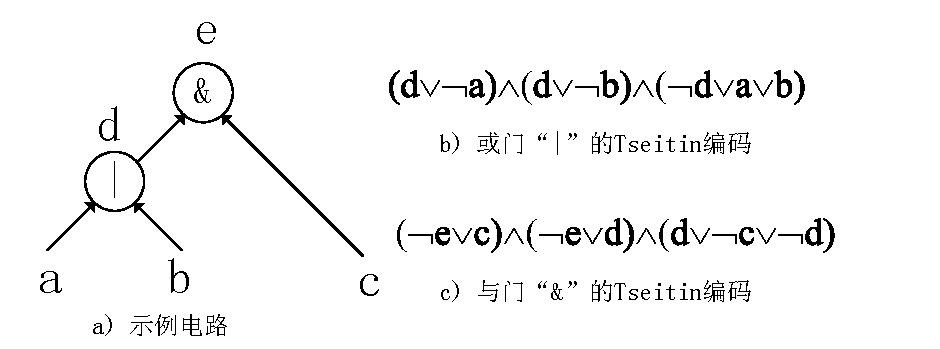
\includegraphics[width=0.8\textwidth]{fig_basic_circuit}
  \caption{示例电路及其编码}
  \label{basic_circuit}
\end{figure}


最简单的SAT求解算法是简单地遍历所有可能的变量赋值,
形成树形的二叉搜索空间。
对于图\ref{basic_circuit}b)的SAT公式,
将导致图\ref{basic_search}所示的二叉搜索树。
其中打钩的叶节点表示合法的求解结果。
每次对特定变量进行二叉分解的步骤称为决策,
每次决策产生一个新的决策层。
图\ref{basic_search}的决策层1、2和3分别对应于分别对变量$a$、$b$和$c$进行二叉分解。

\begin{figure}[t] % use float package if you want it here
  \centering
  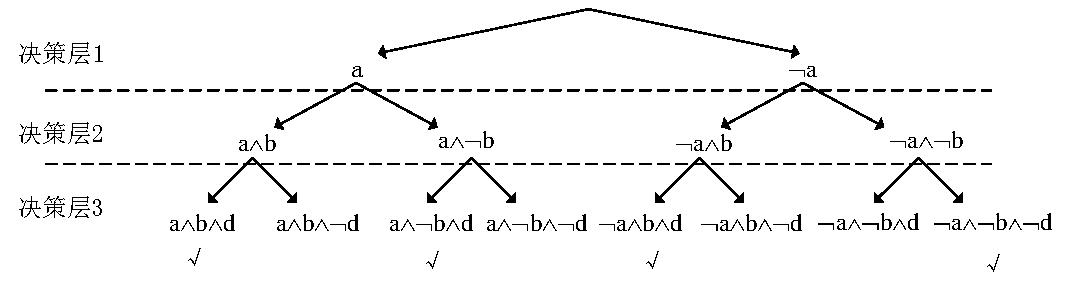
\includegraphics[width=0.8\textwidth]{fig_basic_search}
  \caption{基于完全二叉树遍历的SAT求解}
  \label{basic_search}
\end{figure}

\subsubsection{布尔约束传播(BCP)}
为了使一个特定的SAT公式成立,
必须使其中每个短句都成立。
而为了使某个特定短句成立,
其中必须存在至少一个文字成立。
在某个短句中,
当只有一个特定的文字$w$尚未取值,
而其他所有文字均取值为0,
则该文字必须取值为1。
如果该文字为某个特定变量$v$,
这将导致$v$取值为1,
否则取值为0。
这一推导过程称为布尔约束传播。

以图\ref{basic_circuit}b)的或门的Tseitin编码为例,
为了使该公式成立,
每个短句都必须成立。
以第一个短句$d \wedge a$为例,当$a$ 为1时,
$d \wedge a$化简为$d$,
为了使其成立,
$d$必须取值为1。
此时搜索树如图\ref{BCP}所示。
其中粗线代表在特定决策层内部的BCP 操作。

\begin{figure}[t] % use float package if you want it here
  \centering
  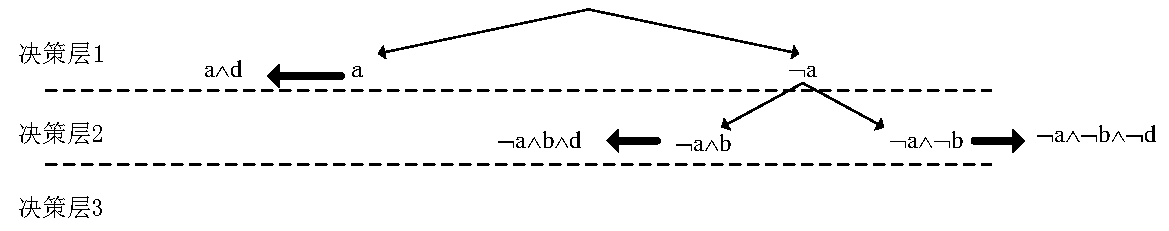
\includegraphics[width=0.8\textwidth]{bcp}
  \caption{布尔约束传播}
  \label{BCP}
\end{figure}

\subsubsection{冲突指导的短句学习}
冲突指导的短句学习和非正交回溯\upcite{CONFLICTLEARN}是提升SAT求解器性能的另一个重要手段。
其中非正交回溯与与本文重点关注的数据结构关系不大,
因此将仅描述冲突指导的短句学习。
为了简明起见,
仍然使用一个例子描述冲突指导的短句学习。
如图\ref{confict}所示的一个二叉搜索树,
当到达红色的标记为conflict 的节点时,
有$\{a \equiv 0,b \equiv 0, c \equiv 0,d \equiv1,e \equiv 0,f \equiv1\}$。
这将导致某个短句中的所有文字均成为0,
称这种情况为一个冲突(conflict)。
此时冲突分析算法将对该短句中的每一个文字,
沿着如图\ref{confict}粗线所示的BCP 关系逆向回溯,
以便找到导致此次冲突的根本原因。
假设找到的三个变量分别为$\{c \equiv 0,d \equiv 1,f \equiv 1\}$,
这意味着a、b和e与本次冲突无关。
无论以后a、b 和e 取任何值,
只要遇到$\{c \equiv 0,d \equiv 1,f \equiv 1\}$ 的情况,
都不必继续搜索。
这意味图\ref{confict}中绿色所示的分支都可以被剪掉。

为了达到这种剪枝效果,
将对冲突分析的结果中每个变量取反,
以构造一个冲突学习短句。
即$\{c \equiv 0, d \equiv 1, f \equiv 1\}$ 将会产生一个冲突学习短句$\{c\vee d \vee \neg f\}$,
并加入短句数组。
以后每次当c、d和f三个变量中的两个满足$\{c \equiv 0, d \equiv 1, f \equiv 1\}$,
则将立即通过冲突学习短句产生一次BCP,
使得第三个变量无法满足$\{c \equiv 0,d \equiv 1,f \equiv 1\}$。
这就构成了一次剪枝操作。

\begin{figure}[t] % use float package if you want it here
  \centering
  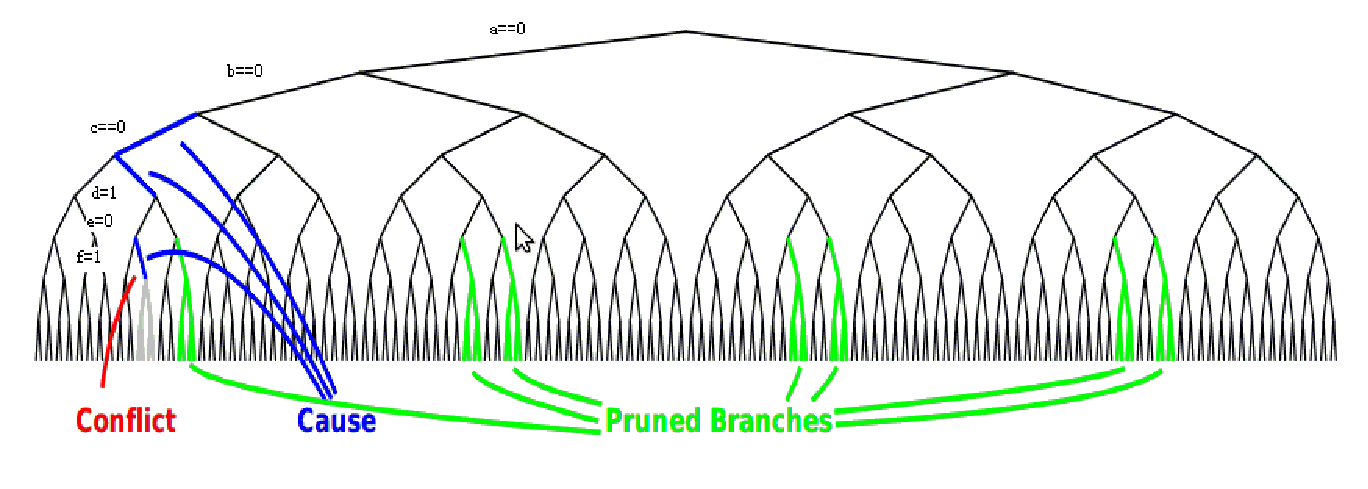
\includegraphics[width=0.8\textwidth]{fig_conflict}
  \caption{冲突指导的短句学习}
  \label{confict}
\end{figure}

\subsubsection{MiniSat 求解器的递增求解机制}\label{subsec_incsat}

本文中,
我们使用MiniSat 求解器\upcite{EXTSAT} 求解所有CNF公式。
和其他基于冲突学习机制\upcite{CONFLICTLEARN}的SAT求解器类似,
MiniSat 从在搜索中遇到的冲突中产生学习短句,
并记录他们以避免类似的冲突再次出现。
该机制能够极大的提升SAT求解器的性能。

在许多应用中,
经常存在一系列紧密关联的CNF公式。
如果在一个CNF公式求解过程中得到的学习短句能够被其他CNF公式共享,
则所有CNF公式的求解速度都能够得到极大的提升。

MiniSat 提供了一个增量求解机制以共享这些学习短句。
该机制包括两个接口函数:
\begin{enumerate}
\item
$addClause(F)$ 用于将一个CNF公式$F$ 添加到MiniSat的短句数据库,
以用于下一轮求解。
\item
$solve(A)$ 接收一个文字集合$A$作为假设,
并求解CNF 公式$F\wedge \bigwedge_{a\in A} a$。
其中$F$是在$addClause$中被加入短句数据库的CNF公式。
\end{enumerate}



\subsection{有限状态机}\label{subsec_fsm}

如图\ref{c2_fsm}a)所示,
本文中编码器使用有限状态机$M=(\vec{s},\vec{i},\vec{o},T)$作为模型。
一个状态机包括状态变量向量$\vec{s}$,
输入变量向量$\vec{i}$,
输出变量向量$\vec{o}$,
和迁移函数$T: [\![\vec{s}]\!]\times [\![\vec{i}]\!]\to [\![\vec{s}]\!]\times [\![\vec{o}]\!]$。
其中$T$用于从当前状态变量向量$\vec{s}$和输入变量向量$\vec{i}$计算出下一状态变量向量$\vec{s}$和输出变量向量$\vec{o}$。

如图\ref{c2_fsm}b)所示,
有限状态机$M$的行为可以通过将迁移函数展开多步得到。
具体的做法是:
\begin{enumerate}
\item 首先使用在小节\ref{subsubsec_tseitin}中描述的Tseitin编码方法,
将迁移函数$T$转化成为对应的CNF公式。
而如图\ref{c2_fsm}b)所示,
我们可以实例化任意多个迁移函数$T$的CNF公式的实例,
同时保证任意两个CNF公式所使用的变量不重叠。
在第n步上,
状态变量$s\in\vec{s}$,输入变量$i\in\vec{i}$ 和输出变量$o\in\vec{o}$
分别表示为$s_n$,$i_n$ 和 $o_n$。
进一步的,
在第n步的状态变量向量,输入变量向量和输出变量向量分别记为$\vec{s}_n$,$\vec{i}_n$ 和 $\vec{o}_n$。

\item 然后对于任意两个相邻的迁移函数$T_n$和$T_{n+1}$,
我们约束$T_n$的次态等于$T_{n+1}$的当前状态,
即都等于图\ref{c2_fsm}b)的$\vec{s}_{n+1}$。
这样任意$n$个迁移函数$T$的实例就能够被连接起来,
形成一个如图\ref{c2_fsm}b)所示长度为$n+1$的序列。
将这些CNF公式的合取形成的新的CNF公式,
送入SAT求解器求解,
所得到的对状态向量序列$<\vec{s}_0,\dots,\vec{s}_n>$的赋值,
就代表了该有限状态机的一个长度为$n$的合法行为。
\end{enumerate}


一条\textbf{路径}是一个状态序列$<\vec{s}_n,\dots,\vec{s}_m>$ 使得$\exists \vec{i}_j\vec{o}_j (\vec{s}_{j+1},\vec{o}_j)\equiv T(\vec{s}_j,\vec{i}_j)$ 对所有$n\le j< m$均满足。
一个\textbf{环}是一条路径$<\vec{s}_n,\dots,\vec{s}_m>$使得$\vec{s}_n\equiv \vec{s}_m$。


\begin{figure}[t]
  \centering
  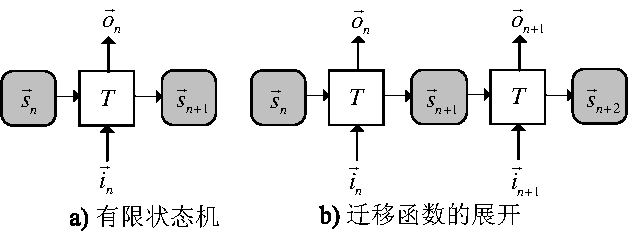
\includegraphics[width=\textwidth]{c2_fsm}
  \caption{有限状态机及其迁移关系的展开}
  \label{c2_fsm}
\end{figure}



\subsection{基于迁移关系(函数)展开的形式化验证算法的一般性原理}\label{subsec_trexp_chap1}
我们已经在上一小节描述了如何将迁移关系(函数)的CNF公式展开成为任意长度的序列。
这种展开方法被广泛应用于绝大多数形式化验证方法中,
以对该状态机的行为进行推理。

假设有待验证的状态机是一个2位计数器,
初始状态为0,
每一步的行为是将当前状态加一。
再假设当计数器为3时会发生一些不希望发生的行为。
因此我们需要验证该计数器永远不会到达3。
因此有待证明的断言是“计数器永远不等于3”。

最简单,
同时也是最典型的限界模型检验\upcite{DBLP:conf/tacas/BiereCCZ99}方法,
通过逐步的增加迁移关系(函数)展开的长度,
以试图找到在展开序列上违反有待证明断言的状态。
比如针对上述“计数器永远不等于3”的断言,
则违反该断言意味着计数器的值等于3.

如图\ref{c2_fsm_exp}所示,
限界模型检验将迁移函数展开了1次,2次和3次。
其中在前2次都没有找到对断言的违反。
而在第3次中则找到了计数器等于3的情况。
在这种情况下,
限界模型检验停止展开,
并给出展开序列上每个状态$\vec{s}^j$的值,
作为反例,
以证明上述“计数器永远不等于3”的断言是错误。

当然,
限界模型检验的算法是不停机的。
即当断言成立的情况下,
无法退出算法。
存在其他方法来部分的改善这一点,
如完备性停机条件\upcite{DBLP:conf/cav/KroeningOSWW11}等。
不过这些方法也都基于上述的基本框架,而且也都有他们自身的缺陷。

\begin{figure}[t]
  \centering
  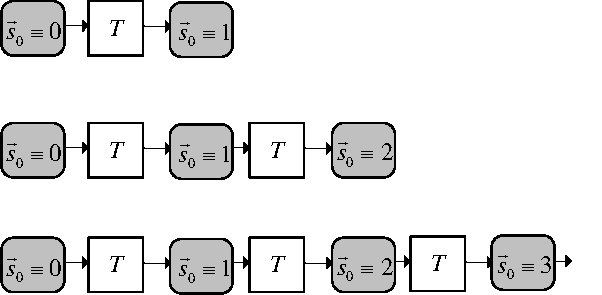
\includegraphics[width=0.8\textwidth]{c2_fsm_exp}
  \caption{一个简单计数器的迁移函数展开序列}
  \label{c2_fsm_exp}
\end{figure}

上述逐步的增加迁移关系(函数)展开长度的框架,
也广泛应用于本文的对偶综合算法中。
详情将在本文的后继部分详细描述。

\section{对偶综合研究现状}\label{sec_now}
本节将简述对偶综合领域取得的研究成果。
由于其中的若干算法也将在本论文的主要章节中被使用,
因此其描述方式根据本论文的需要进行了修改。
因此有可能和原始论文的描述方式有轻微出入。
在阅读本论文时应以本小节的描述为准。

\subsection{早期的充分非完备算法}\label{subsec_sound}

国防科技大学的Shen et al.\upcite{ShenICCAD09}首次提出了对偶综合的概念和初步算法实现。
该算法是充分非完备的,
这意味着当特定编码器对应的解码器存在时,
该算法总能找到其实现;
而当解码器不存在时,
该算法不停机。

该算法类似于小节\ref{subsec_trexp_chap1}中所描述的限界模型检验,
同样是通过逐步的增加迁移函数展开序列的长度,
并在每一个特定长度的展开序列上检查是否存在解码器。


对于每一个$i\in\vec{i}$,
如果存在三个参数$p$, $l$ 和$r$,
使得在长度为$p+l+r$的迁移函数展开序列上,
对于输出序列$<\vec{o}_p,\dots,\vec{o}_{p+l+r}>$的任意取值,
$i_{p+l}$不能同时取值为0和1,
则输入变量$i\in\vec{i}$可以被唯一决定。
这等价于等式(\ref{uniqt1})中的公式$F_{PC}(p,l,r)$的不可满足。

\begin{equation}\label{uniqt1}
% \begin{split}
F_{PC}(p,l,r):=
\left\{
\begin{array}{cc}
&\bigwedge_{m=0}^{p+l+r}
\{
(\vec{s}_{m+1},\vec{o}_m)\equiv T(\vec{s}_m,\vec{i}_m)
\}
\\
\wedge&\bigwedge_{m=0}^{p+l+r}
\{
(\vec{s'}_{m+1},\vec{o'}_m)\equiv T(\vec{s'}_m,\vec{i'}_m)
\}
\\
\wedge&\bigwedge_{m=p}^{p+l+r}\vec{o}_m\equiv \vec{o'}_m \\
\wedge& i_{p+l}\equiv 1 \wedge  i'_{p+l}\equiv 0 \\
\wedge&\bigwedge_{m=0}^{p+l+r}assertion(\vec{i}_m) \\
\wedge&\bigwedge_{m=0}^{p+l+r}assertion(\vec{i'}_m)
\end{array}
\right\}
% \end{split}
\end{equation}

\begin{figure}[t]
\begin{center}
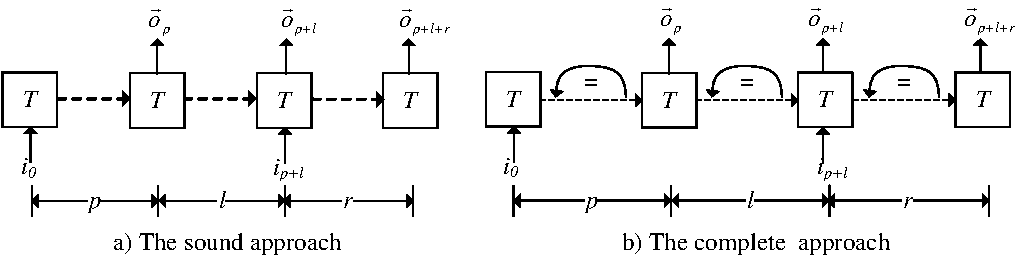
\includegraphics[width=\textwidth]{pc}
\end{center}
\caption{用于检查$i_{p+l}$ 是否能够被唯一决定的充分非完备算法}
  \label{fig_pc_double}
\end{figure}


这里,
$p$是前置迁移函数序列的长度,
$l$ 和$r$则是两个用于唯一决定$i_{p+l}$的输出序列
$<\vec{o}_{p+1},\dots,\vec{o}_{p+l}>$ 和$<\vec{o}_{p+l+1},\dots,\vec{o}_{p+l+r}>$
的长度。
等式(\ref{uniqt1}) 的行1对应于图\ref{fig_pc_double}左边的路径,
而行2对应于图\ref{fig_pc_double}右边的路径。
他们的长度是相同的。
行3强制这两条路径的输出是相同的。
而行4要求他们的输入$i_{p+l}$ 是不同的。
行5和6则是用户给出的断言,
用于约束合法的输入模式。
$F_{PC}$ 中的PC是"parameterized complementary"的缩写,
意味着$F_{PC}(p,l,r)$ 被用于检查在三个参数 $p$,$l$ 和 $r$的情况下,
$i_{p+l}$能否被唯一决定。


从图\ref{fig_pc_double}可知,
等式(\ref{uniqt1}) 的前三行代表了两个具有相同输出的迁移函数展开序列。
因此他们总是可满足的。
而最后两行是对合法输入模式的约束。
我们将在算法开始前检查他们的可满足性。
所以$F_{PC}(p,l,r)$ 的不可满足意味着$i_{p+l}\equiv i'_{p+l}$,
即输入被唯一决定。

从图\ref{fig_pc_double}可知,
如果$F_{PC}(p,l,r)$ 不可满足
则$F_{PC}(p',l',r')$ 对于更大的$p'\ge p$, $l'\ge l$ 和$r'\ge r$也不可满足。
从等式(\ref{uniqt1})中可知,
$F_{PC}(p',l',r')$ 的短句集合是$F_{PC}(p,l,r)$的超集。
这也指向了同一个结论。

这意味着,
$F_{PC}(p,l,r)$的不可满足性的限界证明可以被扩展到
任意$p$, $l$ 和$r$上,
从而成为非限界的证明。

\begin{proposition}\label{prop_pc1}
如果$F_{PC}(p,l,r)$ 不可满足,
则对于任意更大的$p$, $l$ 和$r$,
$i_{p+l}$ 能够被$<\vec{o}_{p},\dots,\vec{o}_{p+l+r}>$ 唯一决定。
\end{proposition}

\begin{algorithm}[t]
\caption{$CheckUniquenessSound(i)$:用于检测$i\in\vec{i}$是否能够被$\vec{o}$的有限长度序列唯一决定的充分算法}
\label{alg_pcsound_chap1}
\begin{algorithmic}[1]
\STATE $p$:= 0;
\STATE $l$:= 0;
\STATE $r$:= 0;
\WHILE {$1$}
\STATE $p$++;
\STATE $l$++;
\STATE $r$++ ;
\IF{$F_{PC}(p,l,r)$ 不可满足}\label{linepc1sound}
\RETURN ($1$,$p$,$l$,$r$)\label{lineln1sound};
\ENDIF
\ENDWHILE
\end{algorithmic}
\end{algorithm}

%

基于上述讨论,
算法\ref{alg_pcsound_chap1}即为我们所提出的充分算法。
该算法首先初始化$p$,$l$和$r$为全0。
然后使用一个循环来持续的增加$p$,$l$和$r$。
在每一个循环中,
将迁移关系展开至长度为$p+l+r$的序列。
若$F_{PC}(p,l,r)$ 不可满足,
则返回当前的$p$,$l$和$r$。


上述算法仅考虑了输入向量$\vec{i}$中的一个输入变量$i$。
当需要讨论整个$\vec{i}$时,
我们需要将整体的$p$, $l$ 和$r$设置为最大值。
即,
假设对于$i\in\vec{i}$,
其对应的唯一决定参数为$p_i$, $l_i$ 和$r_i$,
则对于整个$\vec{i}$,
其对应的唯一决定参数为:
\begin{equation}\label{equ_maxplr}
\begin{array}{ccc}
p & :=  & max_{i\in\vec{i}} \{p_i\}\\
l & :=  & max_{i\in\vec{i}} \{l_i\}\\
r & :=  & max_{i\in\vec{i}} \{r_i\}
\end{array}
\end{equation}

等式(\ref{uniqt1}) 不包含初始状态,
相反使用一个长度为$p$步的前置状态序列$<\vec{s_0},\dots,\vec{s_{p-1}}>$
以将约束$assertion(\vec{i})$传播到状态序列$<\vec{s_p},\dots,\vec{s_{p+l+r}}>$。
从而将在$assertion(\vec{i})$ 约束下不可达的状态集合剔除。
相比考虑初始状态的传统方法,这带来了两个主要的好处:
首先,
通过不计算可达状态,
本文算法可以得到极大的简化和加速。
而相比之下,目前唯一能够计算可达状态的对偶综合算法\upcite{TuDAC13}
则无法处理最为复杂的XFI编码器\upcite{encode6466}。
而我们的算法\upcite{ShenTCAD11}则始终可以处理。
第二,
通过忽略初始状态,本文算法可以产生出更加可靠的解码器。
因为这样可以使得解码器的状态和输出仅仅依赖于有限的输入历史。
因此任何被传输中的错误破坏的$\vec{o}$ 只能对解码器产生有限步数的影响。

当然忽略初始状态有一个缺点在于,
它使得判断条件比必须的情况稍微强一些。
也就是说,
他要求$\vec{i}$ 必须在一个更大的状态集合$R^p$上被唯一决定。
其中$R^p$代表了由任意状态在$p$步之内能够到达的状态集合。
而必要条件是从初始条件出发在任意步数内可以到达的可达状态集合$R$。
因此在某些情况下,
我们的算法有可能无法处理正确设计的编码器。
不过对于目前使用的所有编码器,
即使是那些来自于真实工业应用的编码器,
这种极端情况也没有出现过。


\subsection{完备停机算法}\label{subsec_complete}


在上一小节,
我讨论了当$F_{PC}(p,l,r)$ 不可满足时,
$i_{p+l}$能够针对任意$p$, $l$ 和$r$被唯一决定。
另一方面,
如果$F_{PC}(p,l,r)$ 是可满足的,
则$i_{p+l}$ 不能在特定的$p$, $l$ 和$r$情况下被$<\vec{o}_{p},\dots,\vec{o}_{p+l+r}>$唯一决定。
此时存在两种可能性:
\begin{enumerate}
 \item
在更大的$p$, $l$ 和$r$情况下$i_{p+l}$能够被$<\vec{o}_{p},\dots,\vec{o}_{p+l+r}>$ 唯一决定。
 \item
对任意$p$, $l$ 和$r$,$i_{p+l}$ 都不能够被$<\vec{o}_{p},\dots,\vec{o}_{p+l+r}>$ 唯一决定。
\end{enumerate}

如果是第一种情况,
则通过迭代的增长$p$, $l$ 和$r$,
$F_{PC}(p,l,r)$ 总能够变成不可满足。
然而对于第二种情况,
迭代的递增$p$, $l$ 和$r$将导致不停机。

\begin{figure}[t]
\begin{center}
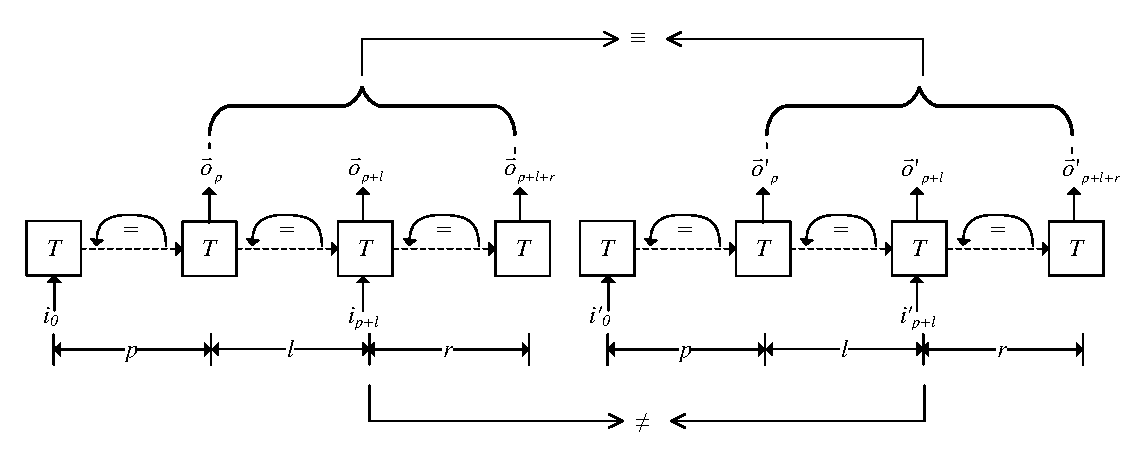
\includegraphics[width=\textwidth]{ln}
\end{center}
\caption{用于检查$i_{p+l}$ 是否不能被唯一决定的上估计算法}
  \label{fig_ln_double}
\end{figure}

因此,
为了得到一个停机算法,
我们需要区分上述两种情形的手段。
国防科技大学的Shen et al.\upcite{ShenTCAD11}和Liu et al.\upcite{LiuICCAD11}分别独立提出了类似的全新的解决方案。
该方案如图\ref{fig_ln_double}所示,
该图类似于图\ref{fig_pc_double},
但是增加了三个约束用于检测三个路径$<\vec{s}_{0},\dots,\vec{s}_{p}>$,$<\vec{s}_{p+1},\dots,\vec{s}_{p+l}>$ 和
$<\vec{s}_{p+l+1},\dots,\vec{s}_{p+l+r}>$上的环。
该方法被形式化的定义于等式(\ref{uniqln}) 中。

\begin{equation}\label{uniqln}
% \begin{split}
F_{LN}(p,l,r):=\\
\left\{
\begin{array}{cc}
&F_{PC}(p,l,r)\\
\wedge&\bigvee_{x=0}^{p-1}\bigvee_{y=x+1}^{p} \{\vec{s}_x\equiv \vec{s}_y\wedge \vec{s'}_x\equiv \vec{s'}_y\} \\
\wedge&\bigvee_{x=p+1}^{p+l-1}\bigvee_{y=x+1}^{p+l} \{\vec{s}_x\equiv \vec{s}_y\wedge \vec{s'}_x\equiv \vec{s'}_y\} \\
\wedge&\bigvee_{x=p+l+1}^{p+l+r-1}\bigvee_{y=x+1}^{p+l+r} \{\vec{s}_x\equiv \vec{s}_y\wedge \vec{s'}_x\equiv \vec{s'}_y\}
\end{array}
\right\}
% \end{split}
\end{equation}

$F_{LN}$ 中的LN意味着环形非对偶。
这表明$F_{LN}(p,l,r)$ 将使用这三个环检测约束来检测$i_{p+l}$是否不能够被唯一决定。

当$F_{LN}(p,l,r)$ 可满足,
则$i_{p+l}$ 不能被$<\vec{o}_{p},\dots,\vec{o}_{p+l+r}>$唯一决定。
更重要的,
通过展开这三个环,
我们能将这个结论扩展到任意更大的$p$, $l$ 和$r$上。
这意味着:

\begin{proposition}\label{prop_ln1}
当$F_{LN}(p,l,r)$ 可满足时,
$i_{p+l}$ 针对任意$p$, $l$ 和$r$都不能被$<\vec{o}_{p},\dots,\vec{o}_{p+l+r}>$ 唯一决定。
\end{proposition}



\begin{algorithm}[t]
\caption{$CheckUniqueness(i)$:用于检测$i\in\vec{i}$是否能够被$\vec{o}$的有限长度序列唯一决定的停机算法}
\label{alg_pcln_chap1}
\begin{algorithmic}[1]
\STATE $p$:= 0;
\STATE $l$:= 0;
\STATE $r$:= 0;
\WHILE {$1$}
\STATE $p$++;
\STATE $l$++;
\STATE $r$++ ;
\IF{$F_{PC}(p,l,r)$ 不可满足}\label{linepc1}
\RETURN ($1$,$p$,$l$,$r$)\label{lineln1};
\ELSIF{$F_{LN}(p,l,r)$ 可满足}\label{lnsat}
\RETURN ($0$,$p$,$l$,$r$);
\ENDIF
\ENDWHILE
\end{algorithmic}
\end{algorithm}

%
%\KwIn{The input variable $i\in\vec{i}$.}
%\KwOut{whether $i\in\vec{i}$ can be uniquely determined by $\vec{o}$, and the value of $p$, $l$ and $r$.}




根据命题\ref{prop_pc1} 和\ref{prop_ln1},
我们能将针对特定$p$, $l$ 和$r$的限界证明扩展到针对任意$p$, $l$ 和$r$的非限界情形。
这使得我们得到停机算法\ref{alg_pcln_chap1},
用于检测$i\in\vec{i}$是否能被$\vec{o}$的有限长度序列唯一决定。
\begin{enumerate}
 \item
一方面,
如果确实存在$p$, $l$ 和$r$,使得输入能被输出唯一决定,
令$p':=max(p,l,r)$,$l':=max(p,l,r)$ 和$r':=max(p,l,r)$。
从命题\ref{prop_pc1},
可知$F_{PC}(p',l',r')$ 是不可满足的。
因此$F_{PC}(p,l,r)$ 总能够在算法\ref{alg_pcln_chap1}行\ref{linepc1}成为不可满足的并退出循环;
 \item
另一方面,
如果不存在这样的$p$, $l$ 和$r$,
则$p$, $l$ 和$r$ 在不断的递增之后最终总能够大于有限状态机的最大无环路径长度。
这意味着在$<\vec{s}_{0},\dots,\vec{s}_{p}>$,$<\vec{s}_{p+1},\dots,\vec{s}_{p+l}>$ 和
$<\vec{s}_{p+l+1},\dots,\vec{s}_{p+l+r}>$上都存在环。
这将使得$F_{LN}(p,l,r)$ 在行\ref{lnsat}被满足。这样将导致退出循环。
\end{enumerate}


因此该算法是停机的。

类似于等式{\ref{equ_maxplr}},
我们需要将整体的$p$, $l$ 和$r$设置为最大值。

\begin{equation}\label{equ_maxplr_ln}
\begin{array}{ccc}
p & :=  & max_{i\in\vec{i}} \{p_i\}\\
l & :=  & max_{i\in\vec{i}} \{l_i\}\\
r & :=  & max_{i\in\vec{i}} \{r_i\}
\end{array}
\end{equation}

\subsection{在对偶综合领域的其他的相关工作}

Shen et al.\upcite{ShenTCAD12}和Liu et al.\upcite{LiuICCAD11} 独立的发现可以通过Craig 插值加速解码器的生成。
该算法还将作为下一章的一部分单独介绍,
因此不在这里展开描述。

Shen et al.\upcite{ShenTCAD12}
通过迭代的剔除所有能导致公式(\ref{uniqln})可满足的配置管脚赋值,
以自动的发掘能够使得解码器存在的前提条件。
如图\ref{multidec}所示,
当 $c_2\equiv 0$时,
常数$20$被赋值到$\vec{o}$。
此时不存在解码器;
当$c_1\equiv 0\wedge c_2\equiv 1$时,
$\vec{i}+1$被赋值到$\vec{o}$,
此时的解码器为$\vec{o}-1$
而当$c_1\equiv 1\wedge c_2\equiv 1$时,
$\vec{i}+2$ 将被赋值到$\vec{o}$。
很明显,
$c_2\equiv 0$首先需要被剔除。
这就得到了$c_2\equiv 1$。
该公式能够使得公式(\ref{uniqt1})不可满足。

然而,
该论文\upcite{ShenTCAD12}首次发现在公式(\ref{uniqt1})不可满足的情况下,
有可能存在多个不同的解码器。
如上述的$c_2\equiv 1$
能够使得公式(\ref{uniqt1})不可满足,
但是此时实际上存在两个解码器。

为了区分所有这些解码器,
该文提出了另一个迭代的算法,
以检查在$c_2\equiv 1$情况下,
公式(\ref{uniqt1})所代表的整体解码器是否能够被分解为目前所发掘的所有解码器的组合。
该检查使用现有的函数依赖算法\upcite{DBLP:journals/tc/JiangLMH10}进行。
当该检查失败时,
所产生的SAT赋值能将公式(\ref{uniqt1})所代表的整体解码器化简为一个尚未被发掘的新解码器。
而当该检查成功时,
为每个解码器所产生的函数依赖公式即为该解码器存在的前提条件。

\begin{figure}[t]
\begin{center}
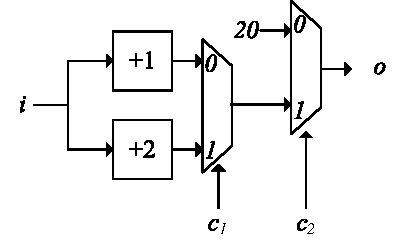
\includegraphics[width=0.35\textwidth]{multidec}
\end{center}
\caption{The encoder used to explain our ideas}
  \label{multidec}
\end{figure}

Tu et al.\upcite{TuDAC13}提出了一个突破性的算法,
基于属性指导的可达性分析算法\upcite{BradleyVMCAI11,EenFMCAD11},
在隐含地而非显式展开的迁移函数序列上,
迭代的精炼归纳不变公式(inductive invariant),
以获得对可达状态的一个单调递减上估计。
如此即可在从$\vec{o}$恢复$\vec{i}$的过程中考虑$\vec{i}$的非限界历史。
该论文针对一些手工构造的例子,
证明了确实存在只有它才能处理的情形。
不过根据我们在来自于真实工业界项目的解码器上的实验,
该算法和我们的算法在处理能力上并没有本质上的区别。



\section{基于白盒模型的对偶综合}\label{sec_whiteboxtodo}
本节阐述基于白盒模型的对偶综合技术的重要研究意义
,并讨论从事该研究所面临的主要挑战
。



%\subsection{研究意义}

现代复杂通讯协议的编码器中,广泛采用了流水线和流控机制\upcite{flowcontrol}技术。
以提高性能并增强对环境的适应能力。
而目前在对偶综合方面的所有研究工作\upcite{ShenICCAD09,ShenTCAD10,ShenTCAD11,ShenICCAD11,ShenTCAD12,LiuICCAD11,LiuTCAD12,TuDAC13}
均基于黑盒模型,
完全忽视上述的内部结构,
从而无法发挥上述内部结构在性能和适应性方面的优势。

\subsubsection{流控机制}
首先,
目前所有对偶综合算法算法\upcite{ShenICCAD09,ShenTCAD10,ShenTCAD11,ShenICCAD11,ShenTCAD12,LiuICCAD11,LiuTCAD12,TuDAC13}的一个前提假设是,
编码器的输入变量$\vec{i}$总能够被输出变量$\vec{o}$的一个有限长度序列唯一决定。

然而,
许多高速通讯系统的编码器带有流控机制\upcite{flowcontrol},
而该机制直接违反了上述假设。
图\ref{fig_nonuniq_chap1}a)展示了一个带有流控机制的通讯系统的结构。
其中一个传输器(transmitter)和一个接收器(receiver)通过一个编码器(encoder)和一个解码器(decoder)连接在一起。
从传输器到编码器有两个输入变量:
有待编码的数据位$d$,
和代表$d$的有效性的有效位$f$。
图\ref{fig_nonuniq_chap1}b)给出了编码器如何将
$f$和$d$映射到输出变量$\vec{o}$的编码表。

流控机制的工作原理为:
\begin{enumerate}
\item
当接收器能够跟上发送器的速度时,
发送器将$f$设为1,
这使得编码器按照$d$的值发送$D_d$。
从图\ref{fig:nonuniq}b)的编码表可知,
解码器总能够根据$D_d$恢复$f$和$d$。
\item
而当接收器无法跟上发送器的速度时,
发送器将$f$设为0以阻止编码器继续发送$D_d$,
转而在不考虑$d$的情况下发送空闲符号$I$。
而解码器应当识别并淘汰$I$,
并将$f\equiv 0$发送给接收器。
此时$d$的具体值并不重要。
\end{enumerate}

上述流控机制能够防止快速发送器发送过多数据以至于接收器无法处理。
然而该机制违反了迄今为止所有对偶综合算法
\upcite{ShenICCAD09,ShenTCAD10,ShenTCAD11,ShenTCAD12,LiuICCAD11,LiuTCAD12,TuDAC13}
的基本假设,
因为在$f\equiv 0$的情况下,
$d$无法被$I$唯一决定。


\begin{figure}
\centerline{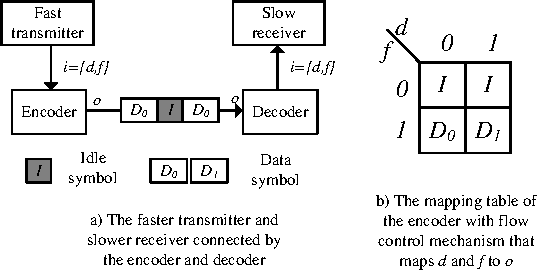
\includegraphics[width=\textwidth]{nonuniq}}
\caption{带有流控机制的通讯系统及其编码器}
\label{fig_nonuniq_chap1}
\end{figure}

因此,
如何在对偶综合算法中处理流控机制,
是一件非常有意义的研究工作。

\subsubsection{流水线结构}

通过研究现有的工业界编码器,我们发现他们都含有流水线结构以提高运行频率。
\begin{figure}[b]
\begin{center}
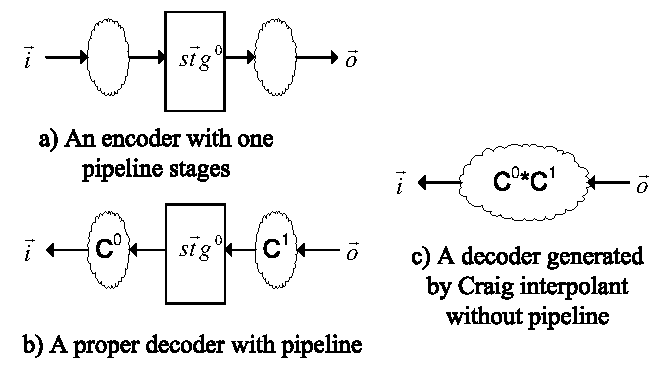
\includegraphics[width=\textwidth]{pipeline_pipeline}
\end{center}
\caption{带有流水线的编码器和解码器}
  \label{fig_pipe_chap1}
\end{figure}

一个带有流水线的简单编码器如图\ref{fig_pipe_chap1}a)所示。
他的关键数据路径被第一级流水线切割成为两段,
从而使得运行频率得到两倍的提升。

他的第一级流水线$\vec{stg}^0$ 包含数个寄存器。
其中输入变量$\vec{i}$ 被用于计算该级流水线$\vec{stg}^0$,
而流水线$\vec{stg}^0$ 则被用于计算$\vec{o}$。
根据该结构,
$\vec{stg}^0$ 能够被$\vec{o}$唯一决定,
而$\vec{i}$ 能够被$\vec{stg}^0$唯一决定。

因此,
一个由人类程序员设计的合理解码器,
应当如图\ref{fig_pipe_chap1}b)所示,
从$\vec{o}$ 中使用组合逻辑$C^1$恢复$\vec{stg}^0$ ,
并进一步使用组合逻辑$C^0$从$\vec{stg}^0$ 中恢复$\vec{i}$ 。
在此类解码器中,
关键路径被流水线级$\vec{stg}^0$切断,
以改善时序。

然而,
目前所有的对偶综合算法\upcite{ShenTCAD11,ShenTCAD12,LiuICCAD11,LiuTCAD12,TuDAC13}
均使用Jiang提出的基于Craig插值\upcite{Craig}的算法 \upcite{InterpBoolFunction}。
如图\ref{fig_pipe_chap1}c)所示,
这些算法从$\vec{o}$中使用一个大型组合逻辑$C^0*C^1$直接恢复$\vec{i}$,
这使得他们变得不必要的很慢,因为没有流水线寄存器切断这段复杂逻辑。

因此,
如何在对偶综合算法中,
产生具有流水线结构的解码器,
是另一件非常有意义的研究工作。



\subsection{面临的挑战}

根据上述研究内容,
目前的算法面临如下挑战:

首先,
在面向流控机制的对偶综合中,需要特征化流控向量上的谓词$valie(\vec{f})$。
而该计算过程中需要对大量冗余变量进行存在量化。
这导致现有解遍历算法无法高效运行,
而基于Craig插值的算法又不支持 \upcite{InterpBoolFunction}对冗余变量进行存在量化。
这就对目前的算法框架提出了严峻挑战。


其次,
在面向流控机制的对偶综合中,
如何扩展目前的算法框架,
使得其基本假设"$\vec{i}$始终能被$\vec{o}$的一个限界序列唯一决定"能够被放松,
以处理流控机制,
是我们所面临的另一个严峻挑战。

再次,
在面向流水线的对偶综合中,
如何推导流水线结构,
并生成带有流水线的解码器,
使我们面临的有一个挑战。

最后,
当上述的流水线和流控机制被混合在一起,
同时出现在同一个编码器中时,
如何同时处理两者及其相互之间的复杂关系,
是本文面临的有一个严峻挑战。






\section{研究内容与创新点}\label{sec_contest_innov}
为了克服上述问题,
本文基于白盒模型,
探索了如何在对偶综合中发掘编码器的内部结构信息,
如流控和流水线结构,
以自动产生支持相应结构的解码器。
本文的主要研究内容及创新点包括以下几方面:

本文受国家自然科学基金项目“面向通讯应用的自动对偶综合方法研究”(项目编号61070132)的支持,主要贡献和创新点如下:



第一,研究了基于余因子(Cofactoring)和Craig插值\upcite{Craig}的迭代特征化算法。
在发掘编码器内部结构和自动产生解码器的过程中,
一个必须而且对性能要求非常苛刻的步骤,
是特征化满足特定命题逻辑关系$R$的布尔函数$f$。
传统的算法包括基于SAT或BDD的完全解遍历和和量词削减。
然而这些算法通常受到解空间不规则的困扰,
导致性能低下。
为此,
我们创造性的提出了一个迭代的特征化算法框架。
在每一次迭代中,
为每一个尚未被遍历的解$A$,
利用其对应的余因子化简$R$以满足产生Craig插值要求。
而该插值是$A$的一个充分扩展。
该迭代过程是停机的,
且其性能比传统的完全解遍历算法有巨大的提升。

第二,研究了针对流控机制的对偶综合算法。
传统对偶综合算法的\upcite{ShenICCAD09,ShenTCAD10,ShenTCAD11,ShenICCAD11,ShenTCAD12,LiuICCAD11,LiuTCAD12,TuDAC13} 的一个基本假设是,
编码器的输入变量$\vec{i}$总能够被输出变量$\vec{o}$的一个有限长度序列唯一决定。
基于该假设方可构造满足Craig插值的不可满足公式。
然而,
许多高速通讯系统的编码器所带有流控机制\upcite{flowcontrol},
直接违反了上述假设。
该机制将$\vec{i}$划分为有待编码的数据向量$\vec{d}$和用以表达$\vec{d}$有效性的流控向量$\vec{f}$,
并在$\vec{f}$上定义一个有效性谓词$valid(\vec{f})$。
只有在$valid(\vec{f})\equiv 1$的情形下,
$\vec{d}$才能够被$\vec{o}$唯一决定。
为此,
我们创造性的提出了能够处理流控机制的对偶综合算法:
\textbf{首先},
它使用经典的对偶综合算法\upcite{ShenTCAD11}
以识别那些能够被唯一决定的输入变量,
并称他们为流控变量$\vec{f}$。
而其他不能被唯一决定的变量称为数据变量$\vec{d}$。
\textbf{第二},该算法推导一个充分必要谓词$valid(\vec{f})$使得$\vec{d}$能够被
输出变量$\vec{o}$的一个有限长度序列唯一决定。
\textbf{第三},
对于每一个流控变量$f\in\vec{f}$,
该算法使用Craig插值算法\upcite{interp_McMillan}特征化其解码器函数。
同时,
对于数据变量$\vec{d}$,
他们的值只有在$valid(\vec{f}) \equiv 1$时才有意义。
因此每个$d\in\vec{d}$的解码器函数可以类似的使用Craig插值算法得到,
唯一的不同在于必须首先应用谓词$valid(\vec{f}) \equiv 1$。



第三,研究了针对流水线结构的对偶综合算法。
现代集成电路中的编码器,
为了提升工作频率,
通常包含多个流水线级,
以将关键的数据路径划分为多级。
而传统的对偶综合算法\upcite{ShenICCAD09,ShenTCAD10,ShenTCAD11,ShenICCAD11,ShenTCAD12,LiuICCAD11,LiuTCAD12,TuDAC13}
完全无视这种流水线结构,
从而导致生成的解码器无法保持和编码器匹配的频率和性能。
为此,
我们创造性的提出了能够产生流水解码器的对偶综合算法:
首先将传统对偶综合算法推广到非输入输出情形,
以找到编码器中每一个流水线级$\vec{stg}^j$中的寄存器集合;
然后使用迭代Craig插值算法特征化每一个流水线级$\vec{stg}^j$的布尔函数,
以从下一个流水线级$\vec{stg}^{j+1}$ 或输出$\vec{o}$之中恢复$\vec{stg}^j$。
最终特征化$\vec{i}$的布尔函数以从
第一个流水线级$\vec{stg}^0$中恢复$\vec{i}$。

第四,结合上述研究成果,研究了能够同时处理流控和流水线结构的对偶综合算法。
该算法首先使用秦et al. \cite{QinTODAES15}的算法来寻找$\vec{f}$ 并推导$valid(\vec{f})$。
然后分别通过强制和不强制$valid(\vec{f})$,
已从所有寄存器集合中找到每一个寄存器级$\vec{stg}^j$的$\vec{d}^j$ 和$\vec{f}^j$。
最后通过Jiang et al. \cite{InterpBoolFunction}的算法特征化$\vec{stg}^j$ 和$\vec{i}$的布尔函数。

综上所述,
本文对基于白盒模型的对偶综合算法中若干关键问题进行了深入的研究,
提出了针对流控和流水线结构的解决方案。
理论分析和实验结果验证了所提出算法的有效性和性能,
对于进一步促进对偶综合算法的发展和应用具有一定的理论意义和应用价值。

\section{论文组织结构}
论文共分八章,组织结构如下:

第一章为绪论,介绍了相关的背景知识,对偶综合的基本概念、特点、应用以及研究现状。分析基于白盒模型的对偶综合技术的研究意义,并简述本文的研究内容和组织结构。

第二章综述了在相关领域的研究成果。

第三章描述了基于余因子和Craig插值\upcite{Craig}的迭代特征化算法。该算法在推导控制流谓词和特征化解码器的布尔函数中被广泛使用。

第四章描述了面向流控机制的对偶综合算法。

第五章描述了面向流水线结构的对偶综合算法。

第六章将上述两个算法有机的结合在一起,能够处理同时包含流控和流水线结构的编码器。

第七章描述了整个试验系统的结构框架,内部各个子系统的功能及相互关系。

第八章总结全文并展望未来的工作。

最后是致谢、博士期间撰写的论文、参加的科研工作以及参考文献。
